\documentclass[t]{beamer}
\usefonttheme{serif}
\usetheme[white]{Wisconsin}
\title{Overview of the Dakota toolkit}
%\subtitle{}
\author{Lucas Jacobson}
\institute{University of Wisconsin--Madison}
\date{20 April 2020}

\usepackage{amsmath}
\usepackage{textcomp}

\newcommand{\tildecenter}{\raisebox{0.5ex}{\texttildelow}}

\begin{document}

% ==============================================================================

\begin{frame}
  \titlepage
\end{frame}

% ==============================================================================

\begin{frame}
  \frametitle{What is Dakota?}
  \begin{itemize}
    \item Robust, usable software for optimization and uncertainty
          quantification (UQ)
    \item Production tool for engineering design and analysis
    \item Research tool for the development of new algorithms
    \item Mainly developed at Sandia National Laboratory
    \item Released as open source under the GNU Lesser General Public License
    \item Website: https://dakota.sandia.gov
  \end{itemize}
\end{frame}

% ==============================================================================

\begin{frame}
  \frametitle{Motivation for initial development}
  \begin{itemize}
    \item Started in 1994 as an internal R\&D activity at Sandia to provide a
          common set of optimization tools for structural analysis problems
    \item Prior to Dakota, there was no effort to archive optimization methods
          for reuse on other projects
    \item Thus, engineers had to build new custom interfaces between engineering
          analysis software and optimization software for each new application
    \item Initial Dakota toolkit provided access to a variety of optimization
          algorithms, hiding the complexity of the underlying software from
          users
    \item Over the years, Dakota has grown to include methods for
    \begin{itemize}
      \item global sensitivity and variance analysis
      \item parameter estimation
      \item uncertainty quantification (UQ)
      \item verification
      \item surrogate-based optimization, hybrid optimization, and optimization
            under uncertainty
    \end{itemize}
  \end{itemize}
\end{frame}

% ==============================================================================

\begin{frame}
  \frametitle{Dakota capabilities}
  \begin{enumerate}[1]
    \item Parameter studies
    \item Design of experiments
    \item Uncertainty quantification
    \item Optimization
    \item Calibration
  \end{enumerate}
  \vskip 0.5in
  \begin{itemize}
    \item These capabilities are described in the succeeding slides
    \item Note: the information in these slides is taken partially verbatim from
          the \href{https://dakota.sandia.gov/content/manuals}{Dakota Version
          6.10 User's Manual}
  \end{itemize}
\end{frame}

% ==============================================================================

\begin{frame}
  \frametitle{Parameter studies}
  \begin{itemize}
    \item Employ deterministic designs to explore the effect of parametric
          changes within simulation models, yielding one form of sensitivity
          analysis
    \item Can help assess simulation characteristics such as smoothness,
          multi-modality, robustness, and nonlinearity, which affect the choice
          of algorithms and controls in follow-on optimization and UQ studies
    \item Typical examples include centered, one-at-a-time variations or joint
          variation on a grid
  \end{itemize}
\end{frame}

% ==============================================================================

\begin{frame}
  \frametitle{Design of experiments}
  \begin{itemize}
    \item Acronym: design and analysis of computer experiments (DACE) techniques
    \item Used to explore the parameter space of an engineering design problem,
          for example to perform global sensitivity analysis
    \item Can help reach conclusions similar to parameter studies, but the
          primary goal of these methods is to generate good coverage of the
          input parameter space
    \item Representative methods include Latin hypercube sampling, orthogonal
          arrays, and Box-Behnken designs
  \end{itemize}
\end{frame}

% ==============================================================================

\begin{frame}
  \frametitle{Uncertainty quantification}
  \begin{itemize}
    \item Also referred to as nondeterministic analysis methods
    \item Compute probabilistic information about response functions based on
          simulations performed according to specified input parameter
          probability distributions
    \item Perform a forward uncertainty propagation in which probability
          information for input parameters is mapped to probability information
          for output response functions
    \item Approaches include Monte Carlo sampling, reliability methods, and
          polynomial chaos expansions
  \end{itemize}
\end{frame}

% ==============================================================================

\begin{frame}
  \frametitle{Optimization}
  \begin{itemize}
    \item Minimize cost or maximize system performance, as predicted by the
          simulation model, subject to constraints on input variables or
          secondary simulation responses
    \item Categories of algorithms include gradient-based, derivative-free, and
          global optimization
    \item Dakota also includes capabilities for multi-objective trade-off
          optimization and automatic scaling of problem formulations
    \item Advanced Dakota approaches include hybrid (multi-method), multi-start
          local, and Pareto-set optimization
  \end{itemize}
\end{frame}

% ==============================================================================

\begin{frame}
  \frametitle{Calibration}
  \begin{itemize}
    \item Maximize agreement between simulation outputs and experimental data
          (or desired outputs)
    \item Solve inverse problems (often referred to as parameter estimation or
          least-squares problems)
    \item Dakota approaches include nonlinear least squares and Bayesian
          calibration
  \end{itemize}
\end{frame}

% ==============================================================================

\begin{frame}
  \frametitle{Related advanced capabilities}
  \begin{itemize}
    \item Surrogate models
    \begin{itemize}
      \item Inexpensive approximate models that aim to capture the features of
            an expensive high-fidelity model
      \item Include data fits, multifidelity, and reduced-order model surrogates
      \item Can serve as inexpensive stand-ins for optimization or UQ studies
    \end{itemize}
    \item Nested models
    \begin{itemize}
      \item Permit layering one Dakota method over another
      \item Enable methods like mixed epistemic-aleatory or second-order UQ,
            optimization under uncertainty, or surrogate-based UQ
    \end{itemize}
    \item Solution verification and Bayesian calibration/UQ
    \item Parallel computing
    \begin{itemize}
      \item Dakota is designed to exploit parallel computing resources
    \end{itemize}
    \item GUI
    \begin{itemize}
      \item Intuitively link Dakota study to simulation model
      \item Graphically plot output data from Dakota study
    \end{itemize}
  \end{itemize}
\end{frame}

% ==============================================================================

\begin{frame}
  \frametitle{Coupling Dakota to a simulation}
  \begin{figure}
    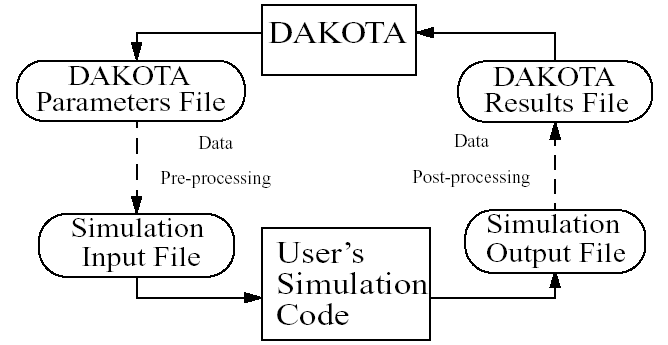
\includegraphics[scale=0.3]{images/blackbox.png}
  \end{figure}
  \begin{itemize}
    \item Single, simple interface between Dakota and user's simulation code
    \item Easy to try new methods or algorithms; generally only need to change a
          few lines in the Dakota text input file
    \item Does not require deep knowledge of underlying Dakota software packages
    \item ``Black-box'' coupling: Dakota and user's simulation code
          exchange data by reading and writing short text files
    \item Closer coupling is possible for advanced users if needed
  \end{itemize}
\end{frame}

% ==============================================================================

\end{document}
